\documentclass[12pt]{article}
\usepackage{graphicx}
\usepackage{float}
\usepackage{amsmath}
\usepackage{amsfonts}
\usepackage[brazilian]{babel}
\usepackage[utf8]{inputenc}
\usepackage[T1]{fontenc}

\begin{document}

\title{Funções: Exercícios Complementares}
\author{Erik Perillo}
\date{}
\maketitle

\newpage

\section{Exercícios}
\begin{enumerate}
	\item Um dentista descobriu que uma pessoa em média tem 4 cáries. 
		Além disso, para cada quilo de açúcar que uma pessoa consome por mês,
		a pessoa tem uma cárie a mais. O dentista agora quer uma função $f(x)$
		que descreva quantas cáries uma pessoa tem de acordo com quantos quilos
		de açúcar ela consome.
	\begin{enumerate}
		\item O que $f(x)$ representa neste caso?
		\item O que a variável independente ($x$) representa neste caso?
		\item Qual a relação entre as quantidades dos itens a) e b)?
		\item O dentista descobriu 6 cáries em uma pessoa. Quantos quilos de 
			açúcar ela deve consumir por mês?
	\end{enumerate}

	\item Um homem tem $8$ mil seguidores no \textit{twitter}. Ele postou 
		um twitt negativo sobre a Cláudia Leitte e seus fãs não gostaram. Ele
		está perdendo 3 seguidores a cada segundo por causa da sua postagem.
		Agora ele quer saber quantos seguidores ele tem de acordo com os 
		segundos que se passaram.
	\begin{enumerate}
		\item Qual a quantidade de interesse dele?
		\item Do que essa quantidade de interesse depende?
		\item Como elas se relacionam?
		\item Escreva a função $f(x)$.
		\item Desenhe-a no gráfico.
		\item Quantos segundos vão se passar até que ele tenha 8 seguidores?
		\item Depois de 24 horas, quantos seguidores ele terá?
	\end{enumerate}

	\item Uma motociclista descobriu que sua moto anda 8km a cada litro de
		gasolina que ela põe na moto. O litro da gasolina está custando 
		R\$3,55. A motociclista quer saber quantos km ela vai poder andar 
		com sua moto de acordo com quanto dinheiro ela põe em gasolina por
		meio de uma função $f(x)$.
	\begin{enumerate}
		\item O que $f(x)$ representa nesse caso?
		\item O que a variável independente ($x$) representa?
		\item Qual a relação entre as quantidades dos itens a) e b)?
		\item Escreva a função $f(x)$.
		\item Quanto ela vai ter que gastar para poder andar 45km?
		\item Desenhe o gráfico da função.
	\end{enumerate}
\end{enumerate}

\newpage

\section{Respostas aos Exercícios}
\begin{enumerate}
	\item 
	\begin{enumerate}
		\item O número de cáries.
		\item O número de quilos de açúcar que uma pessoa consome por mês.
		\item A cada um quilo de açúcar, a pessoa tem uma cárie a mais. Além
			disso, a pessoa já tem 4 cáries sempre. Assim, podemos dizer que 
			$f(x)$, o número de cáries que uma pessoa tem, é $4 + x$.
		\item $f(x) = 6 \implies 4 + x = 6 \implies x = 2$
	\end{enumerate}

	\item 
	\begin{enumerate}
		\item O número de fãs.
		\item De quantos segundos se passaram desde o post negativo.
		\item Ele tem 90 mil seguidores de início e, a cada um segundo, 
			perde três.
		\item $f(x) = 90000 - 3x$
		\item --
			\begin{figure}[H]
				\centering
				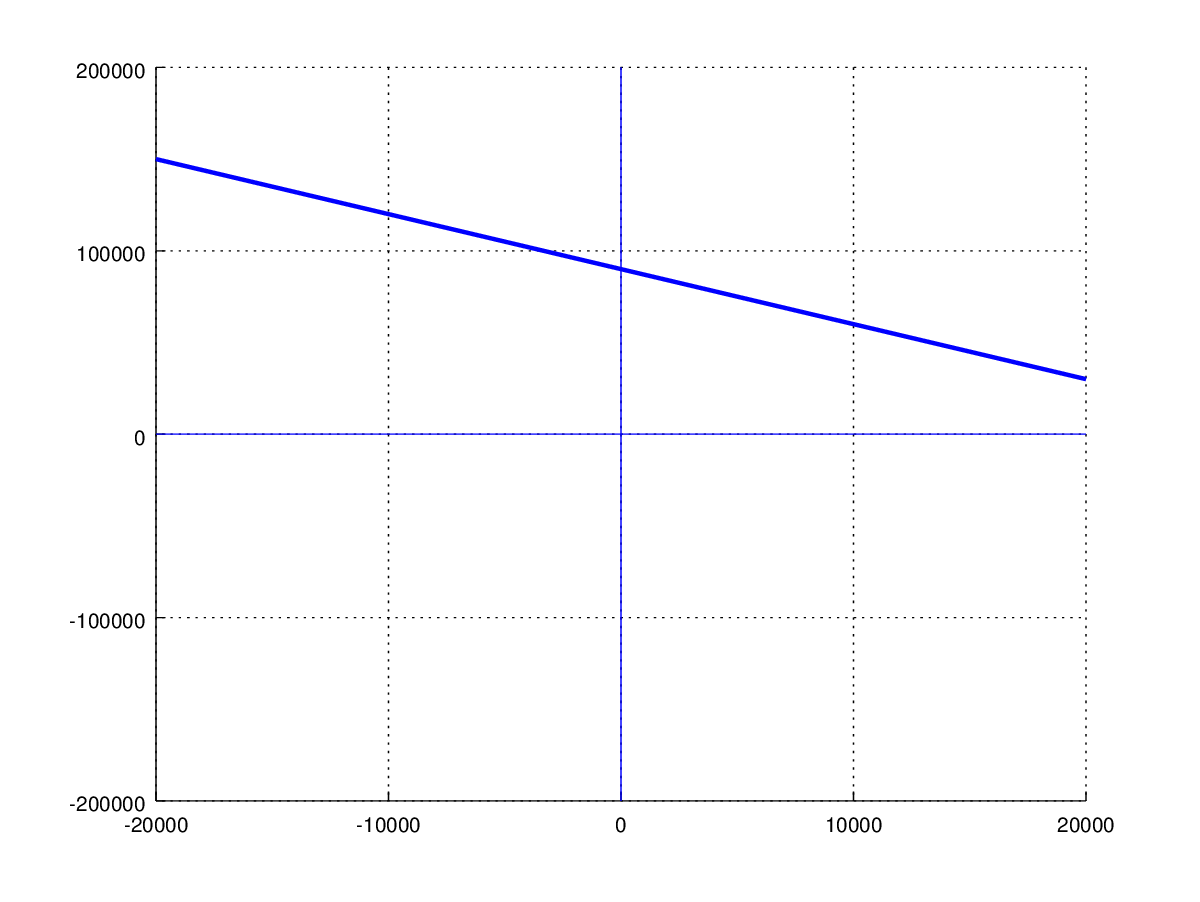
\includegraphics[width=0.8\linewidth]{imgs/exc2chart.png}
			\end{figure}
		\item $f(x) = 8 \implies 90000 - 3x = 8 \implies x = 
			\frac{(8 - 90000)}{-3} = 29997.333$
		\item 6 horas são $6*60 = 360$ minutos. 360 minutos são 
		$360*60 = 21600$ segundos. Assim, $f(21600) = 90000 - 21600*3 =
		25200$
	\end{enumerate}

	\item 
	\begin{enumerate}
		\item Quantos km ela consegue andar.
		\item Quantos reais ela gasta na gasolina.
		\item A cada um real que ela gasta em gasolina, ela pode andar 2km.
		\item $f(x) = 2x$
		\item $f(x) = 54 \implies 54 = 2x \implies x = 54/2 = 27$
		\item --
			\begin{figure}[H]
				\centering
				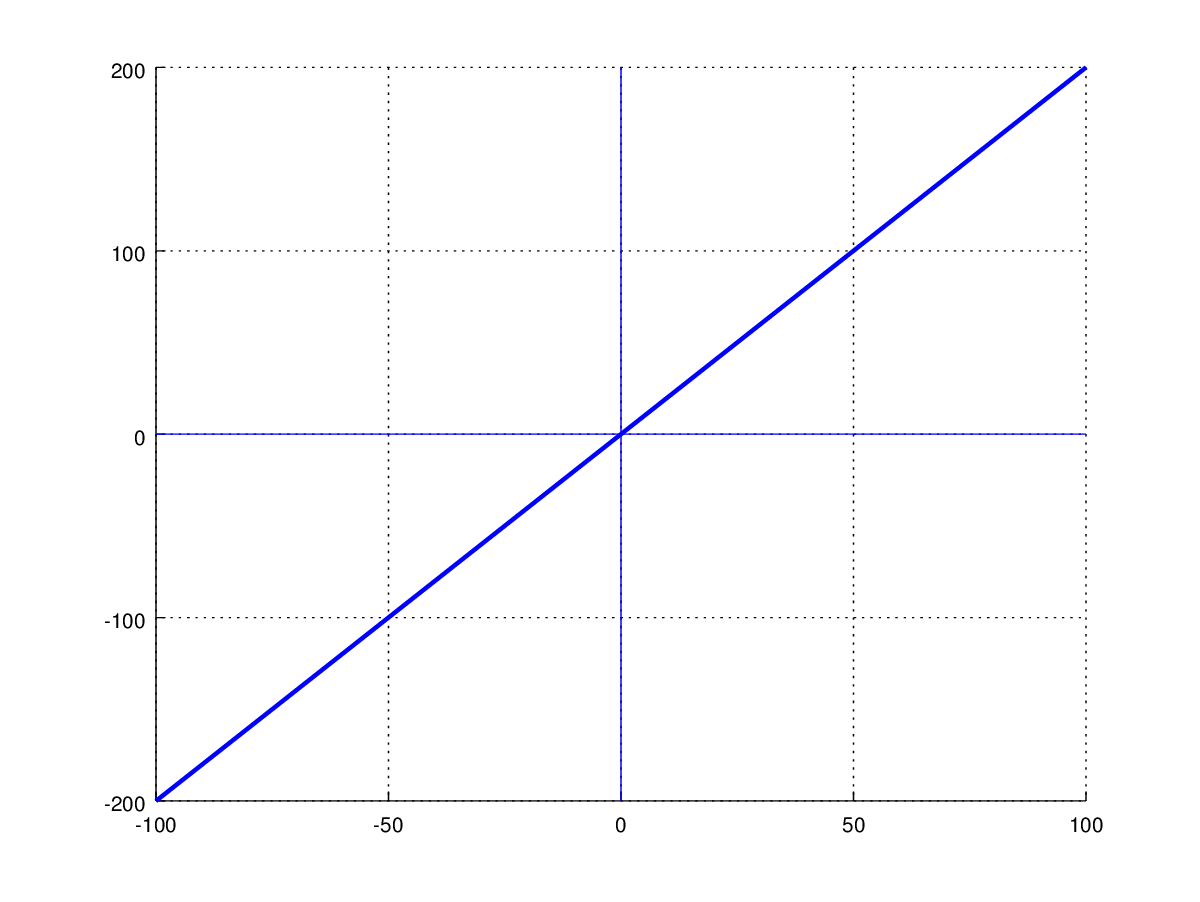
\includegraphics[width=0.8\linewidth]{imgs/exc2chart2.png}
			\end{figure}
	\end{enumerate}
\end{enumerate}

\end{document}
